%----- Jan:

%- gewichtung motivieren

\begin{frame}{Acceptance/Efficiency Maps}

\begin{block}{Muon Acceptance}
\begin{itemize}
\item evaluated in $N(\si{jets})$- and $\slashed H_{\si{T}}$-bins
\item acceptances highly dependant on bin
\end{itemize}
\end{block}

\begin{center}
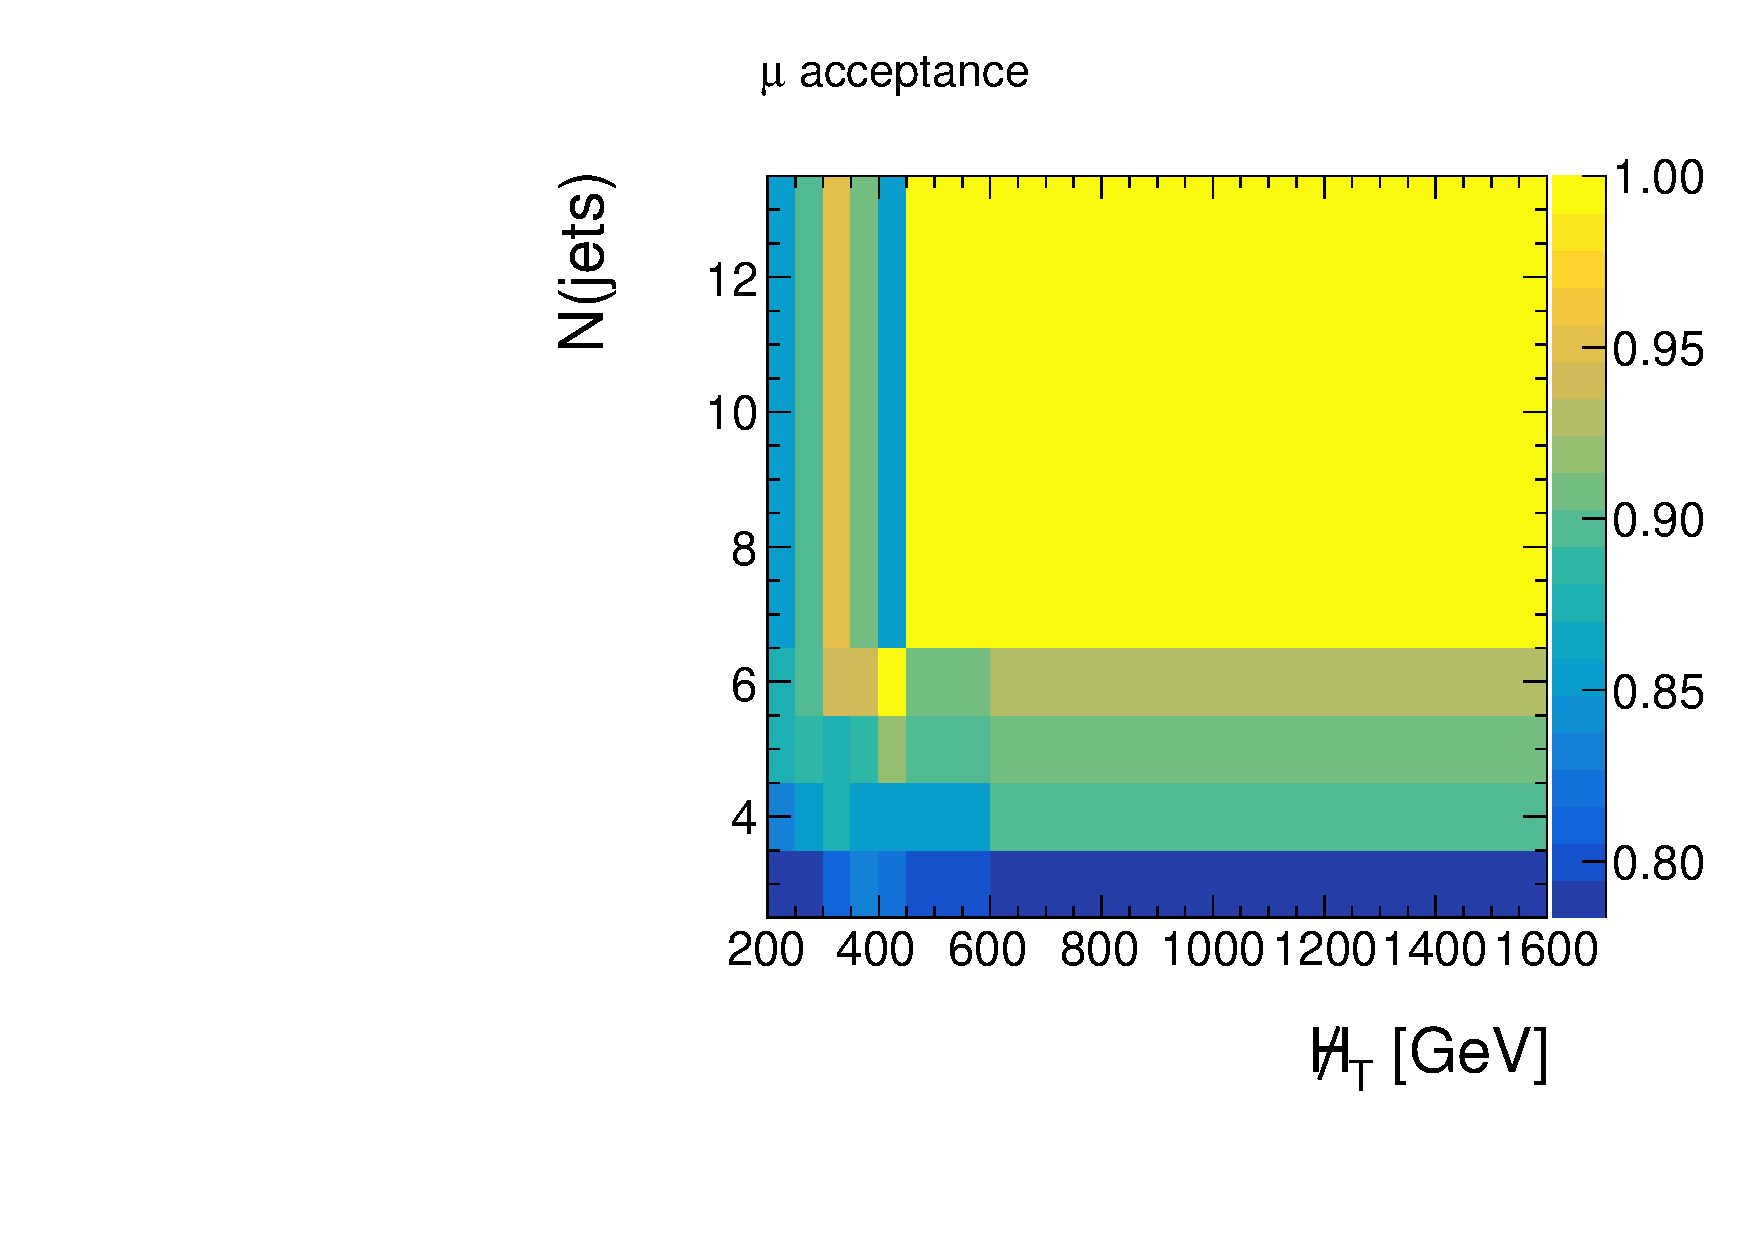
\includegraphics[width = 0.5 \textwidth]{plots11/MuonAcceptance.pdf}
\end{center}

\end{frame}


\begin{frame}{Acceptance/Efficiency Maps}

\begin{block}{Reconstruction Efficiency}
\begin{itemize}
\item only events that pass muon acceptance are considered
\item evaluated in $N(\si{jets})$-, $H_{\si{T}}$- and $\slashed H_{\si{T}}$-bins
\item efficiencies also highly dependant on bin
\end{itemize}
\end{block}

\begin{center}
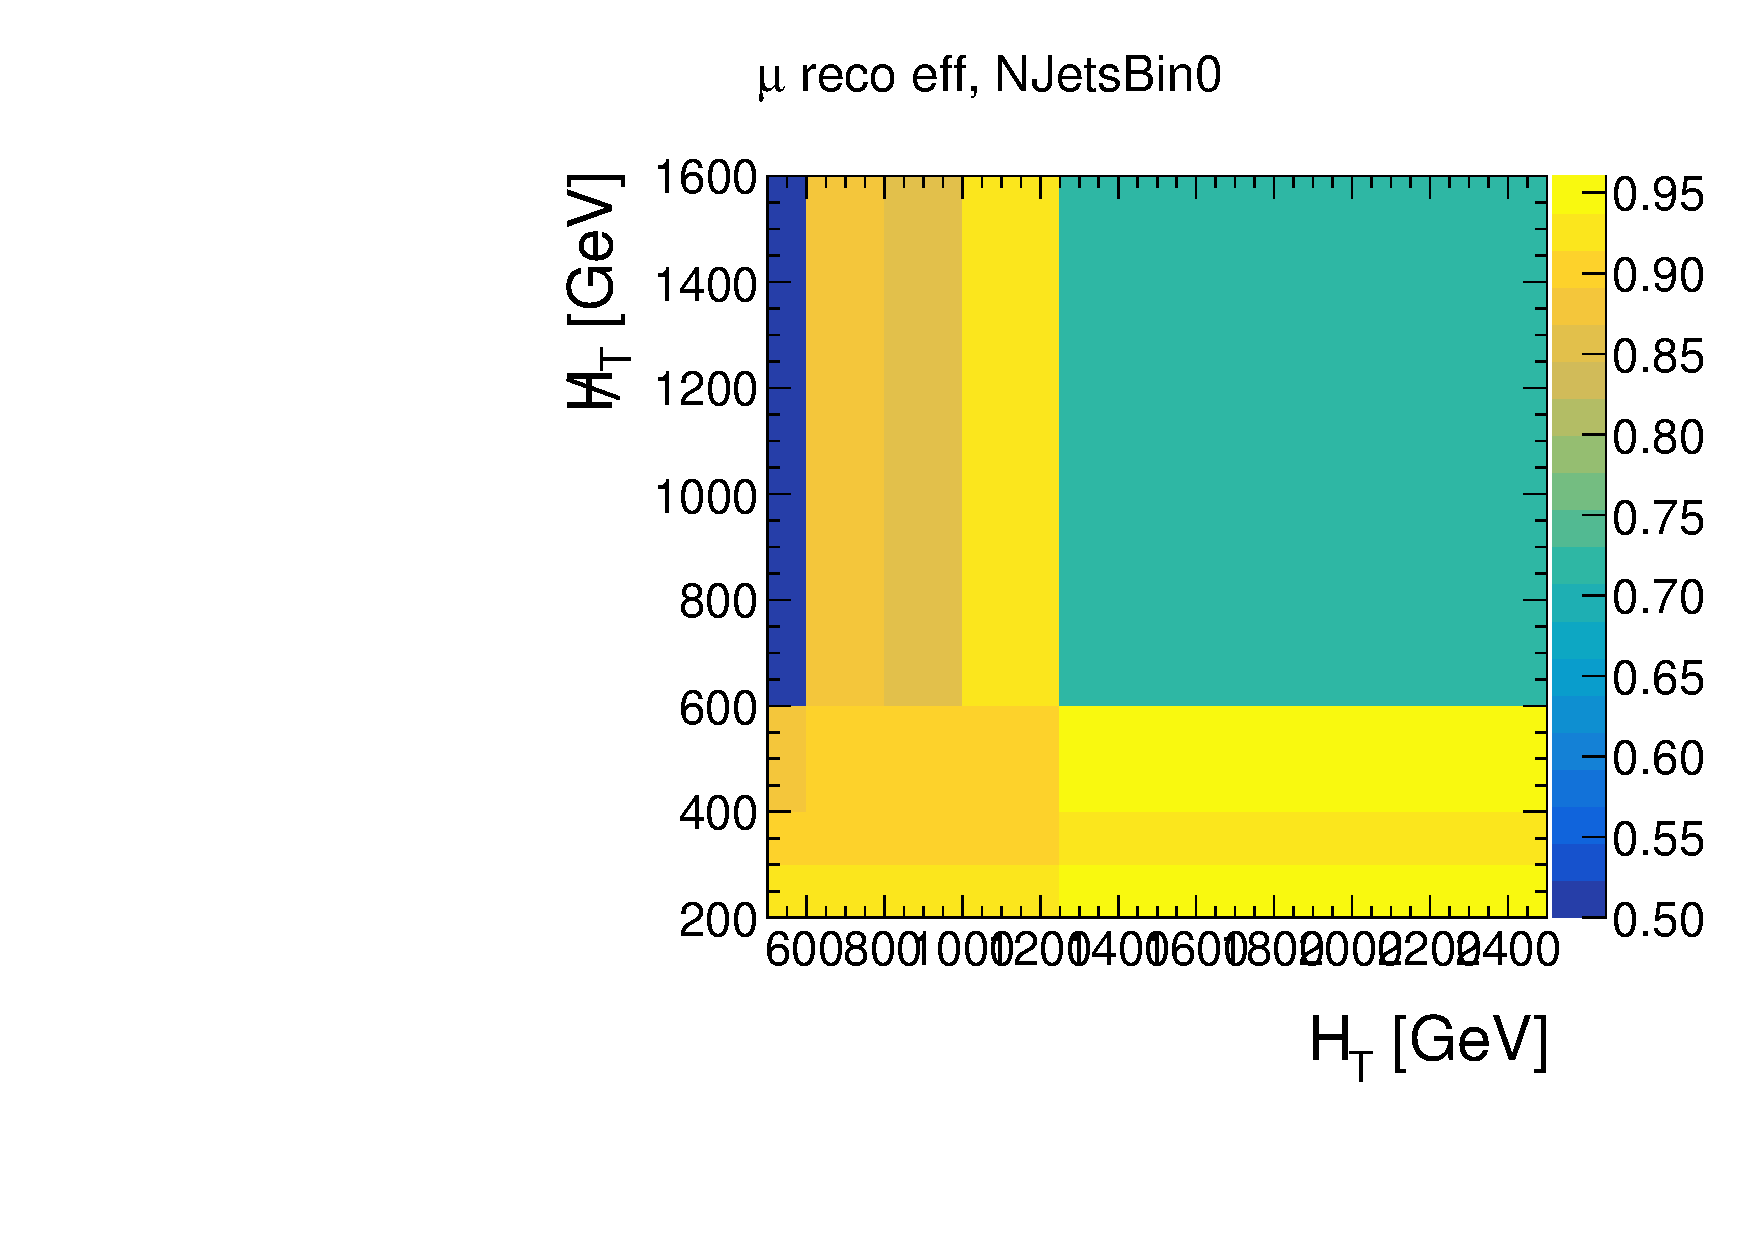
\includegraphics[width = 0.4\textwidth]{plots11/MuonRecoEff_NJetsBin0.pdf}
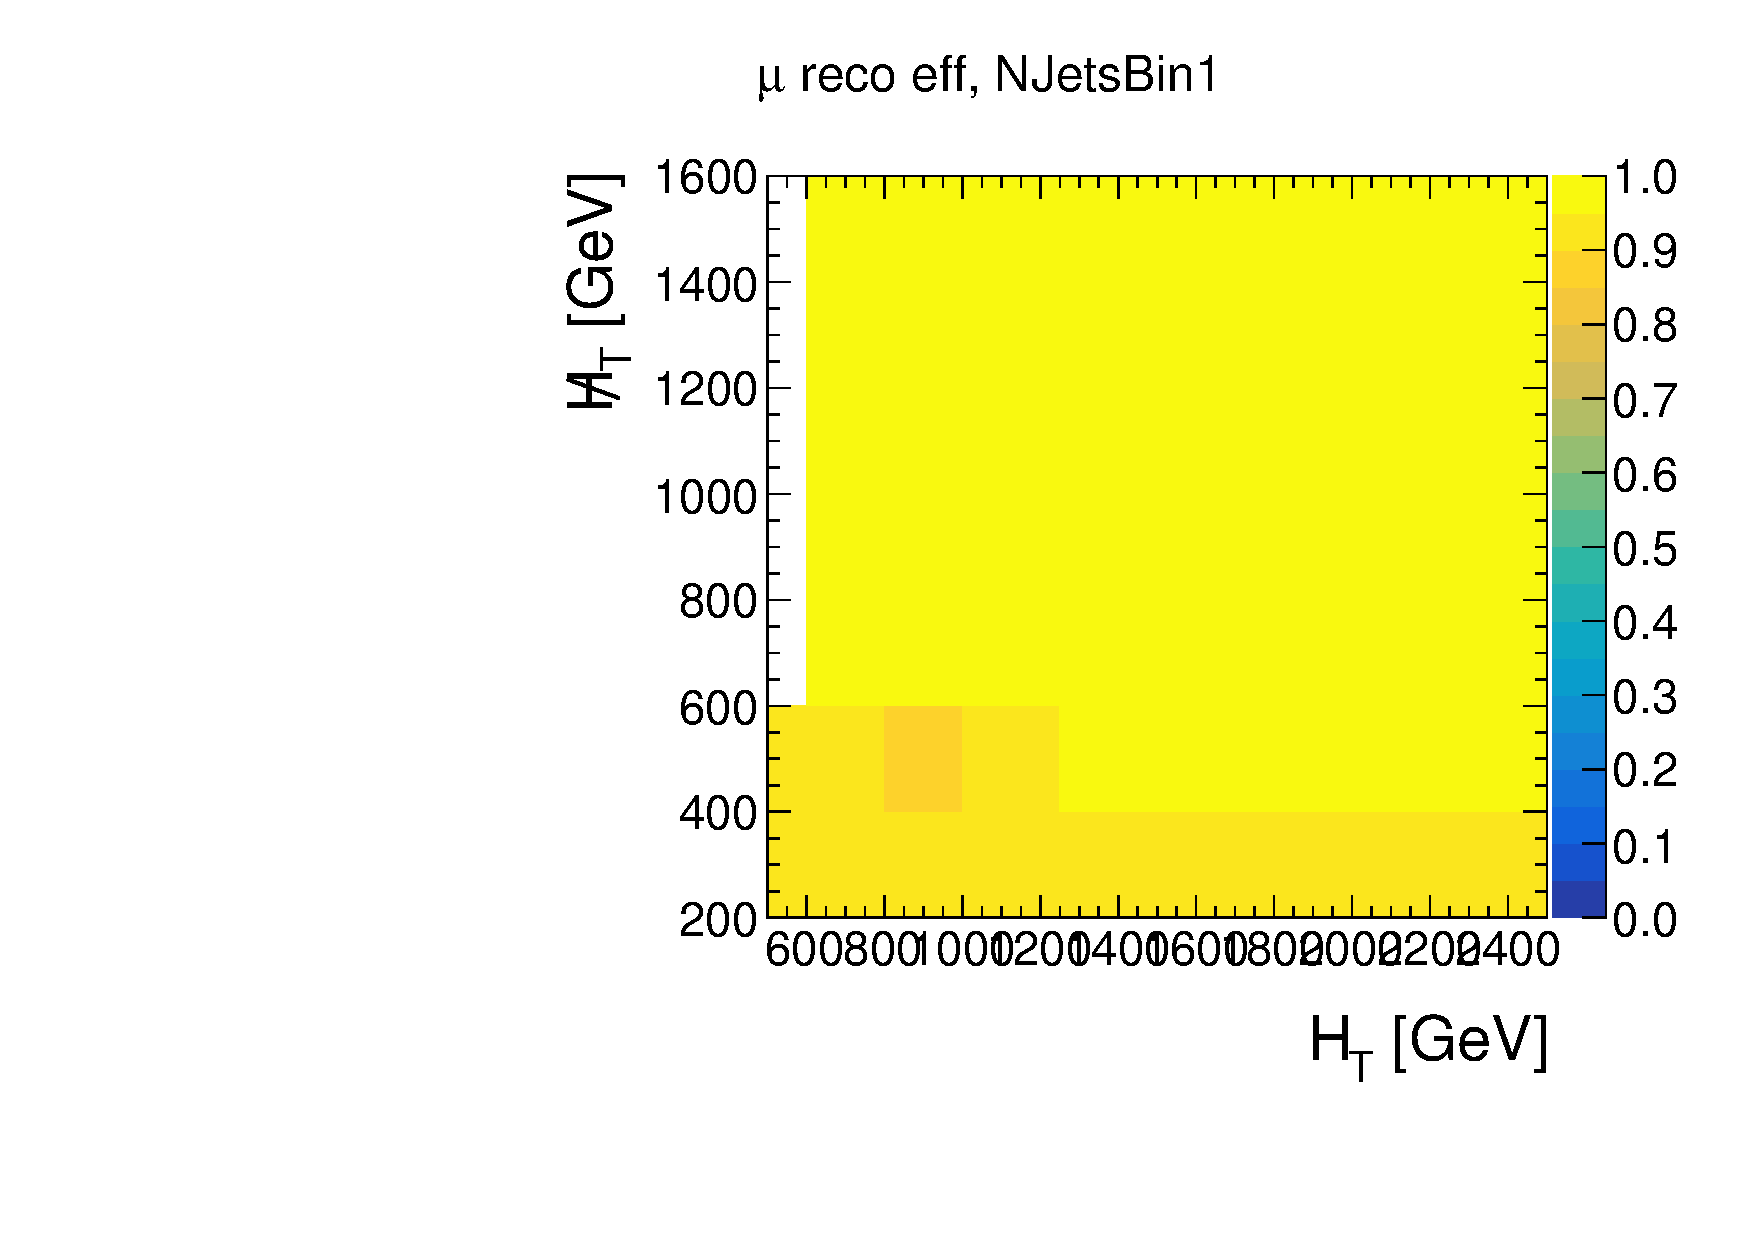
\includegraphics[width = 0.4\textwidth]{plots11/MuonRecoEff_NJetsBin1.pdf}
\end{center}

\end{frame}


%- closure test
\begin{frame}{Validation of the Implemented Method}

\begin{block}{Closure Test}
\begin{itemize}
\item apply self-implemented method to W+jets MC sample\\
\begin{itemize}
	\item cut sample to events with one isolated $\mu$ (control sample)
	\item weight events with probability that $\mu$ is not isolated\\
	$\Rightarrow$ mimic distribution where no isolated $\mu$ found 
\end{itemize}
\item compare to sample where falsely no isolated $\mu$ was found
\end{itemize}
\end{block}

\begin{center}
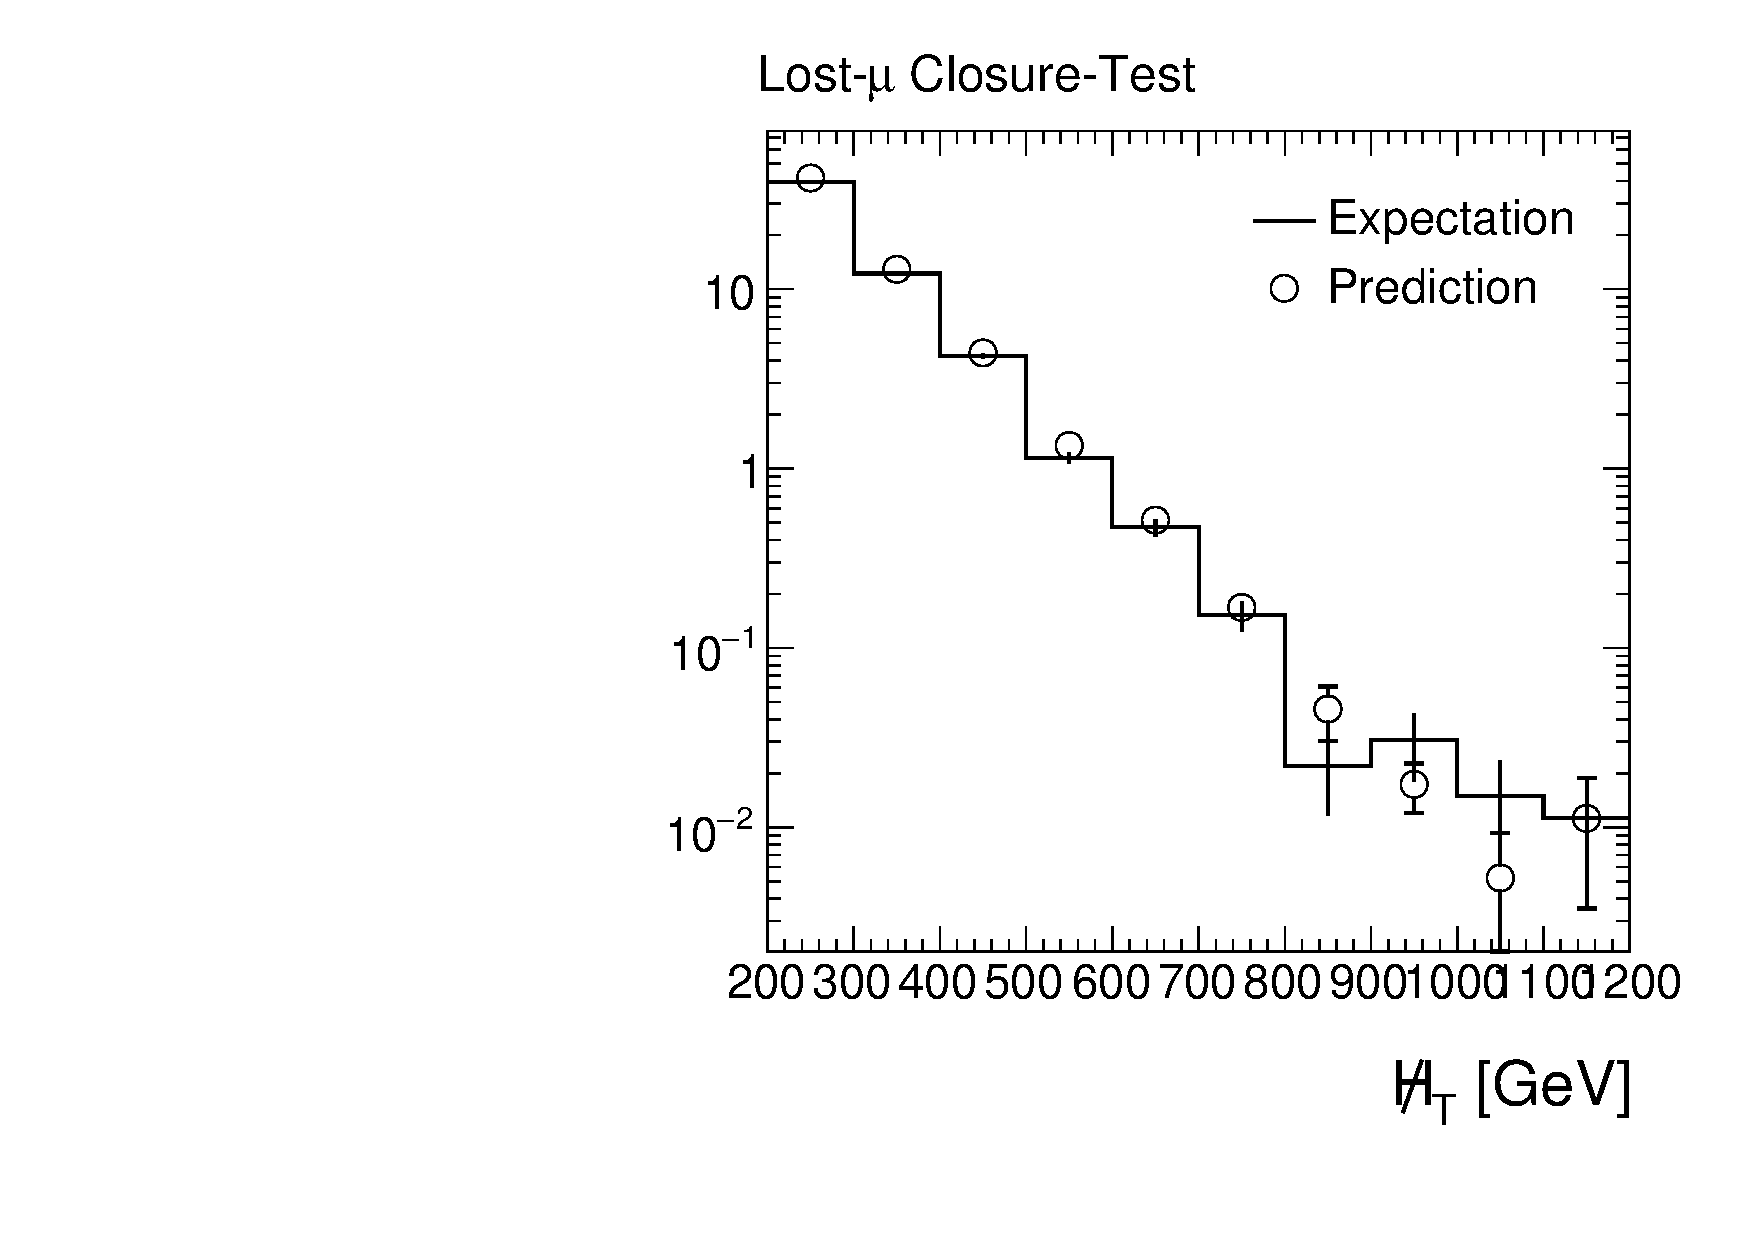
\includegraphics[width = 0.37\textwidth]{plots11/LLClosureMHT.pdf}
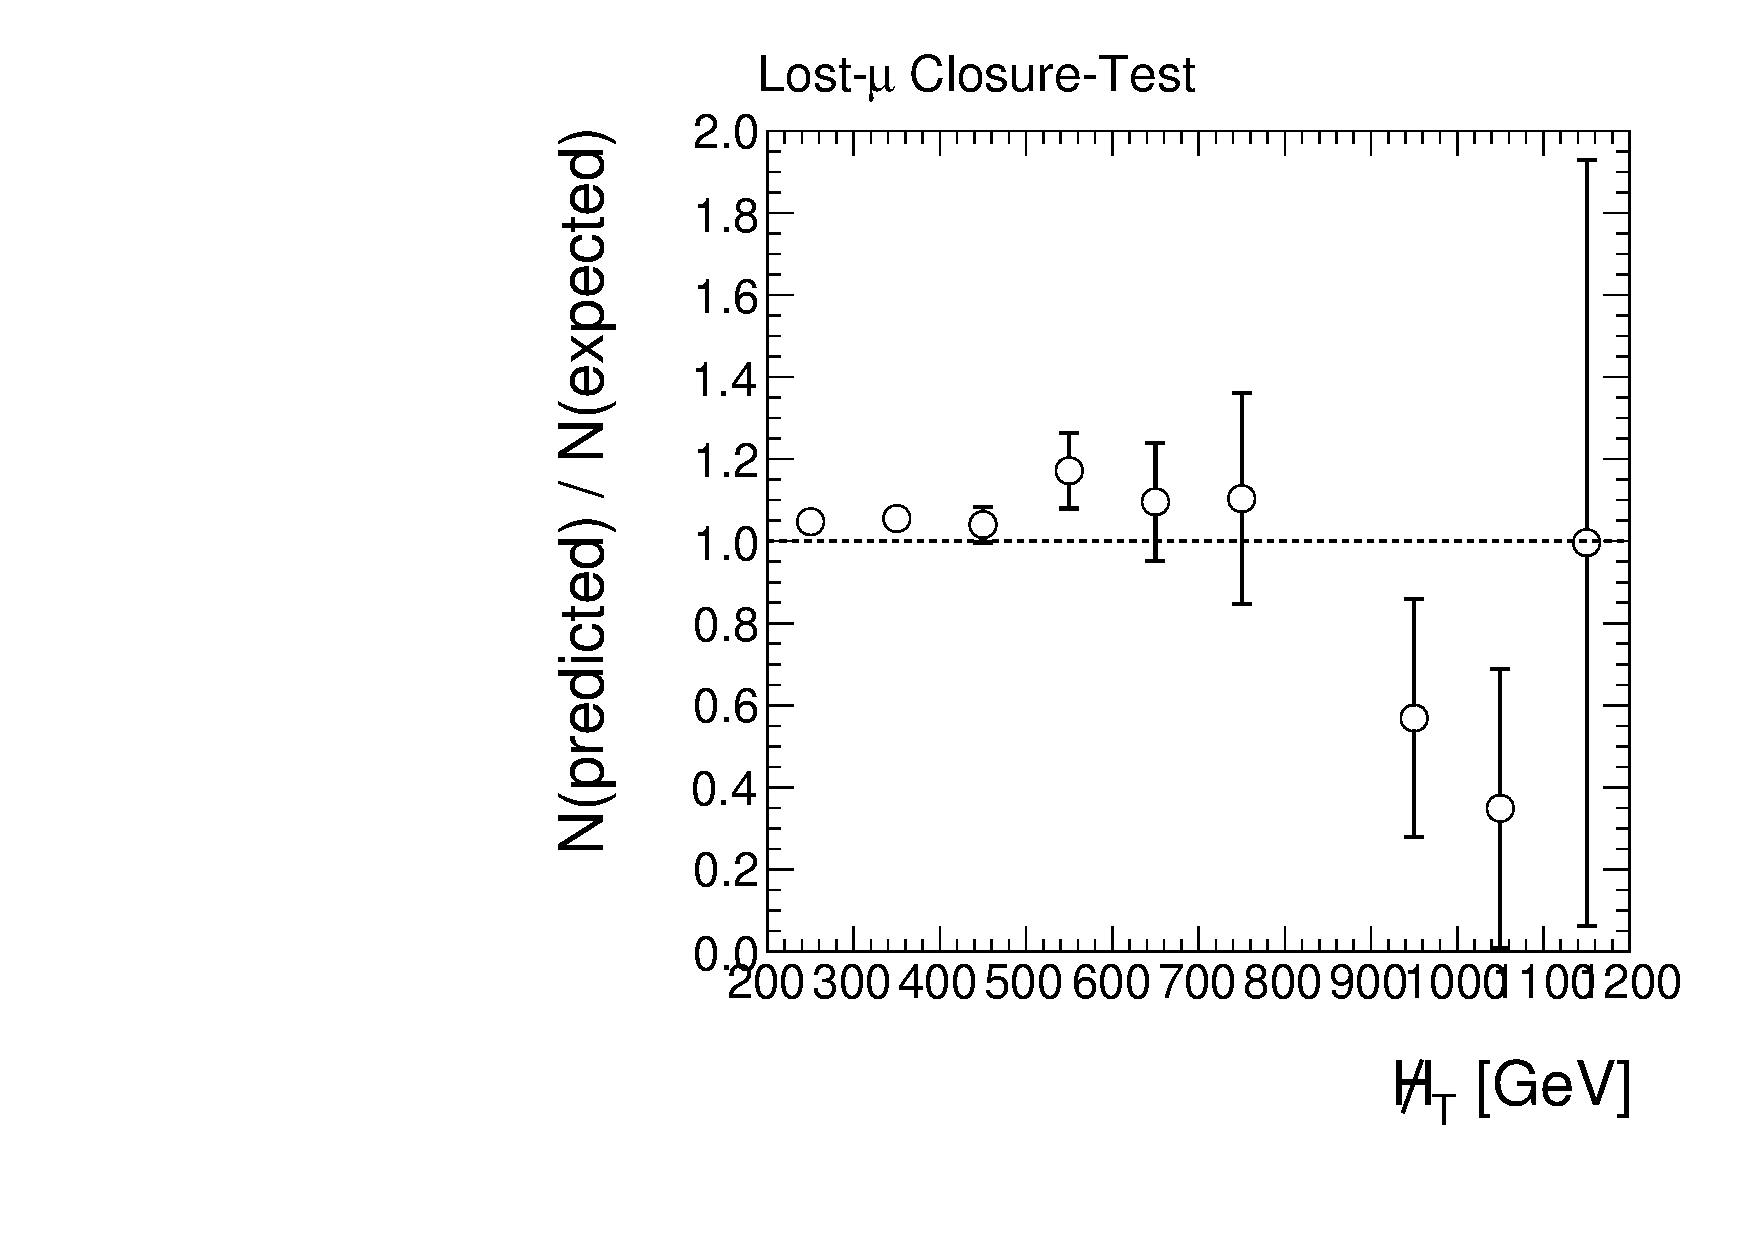
\includegraphics[width = 0.37\textwidth]{plots11/LLClosureMHTRatio.pdf}
\end{center}

\end{frame}


\begin{frame}{Predict Background from Data}

\begin{block}{Method}
\begin{itemize}
\item generate new efficiency maps for full lost-lepton method
\begin{itemize}
	\item consider lost electrons
	\item consider $\mathsf{t\overline{t}}$+jets events
\end{itemize}
\item apply efficiency weighting to data
\end{itemize}
\end{block} 

\begin{center}
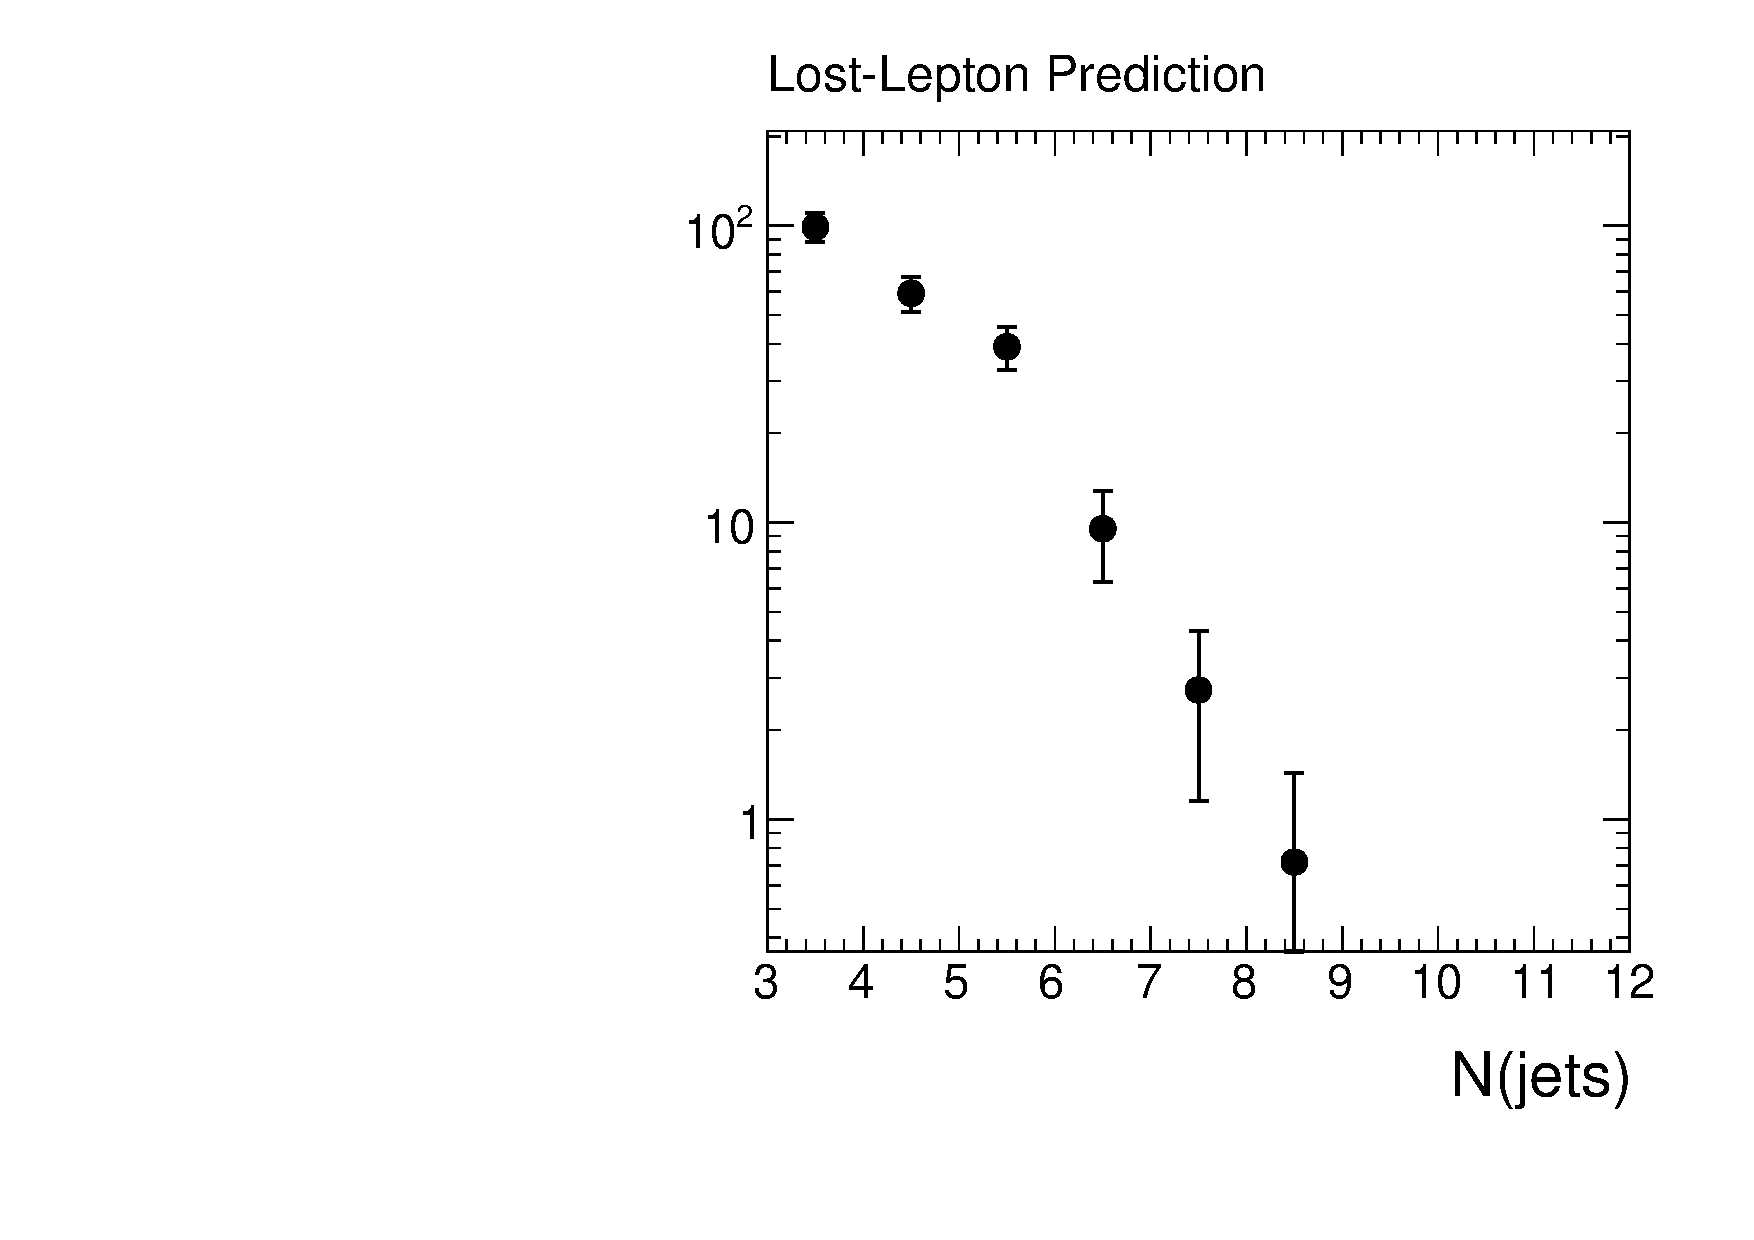
\includegraphics[width = 0.4\textwidth]{plots11/LLPredictionNJets.pdf}
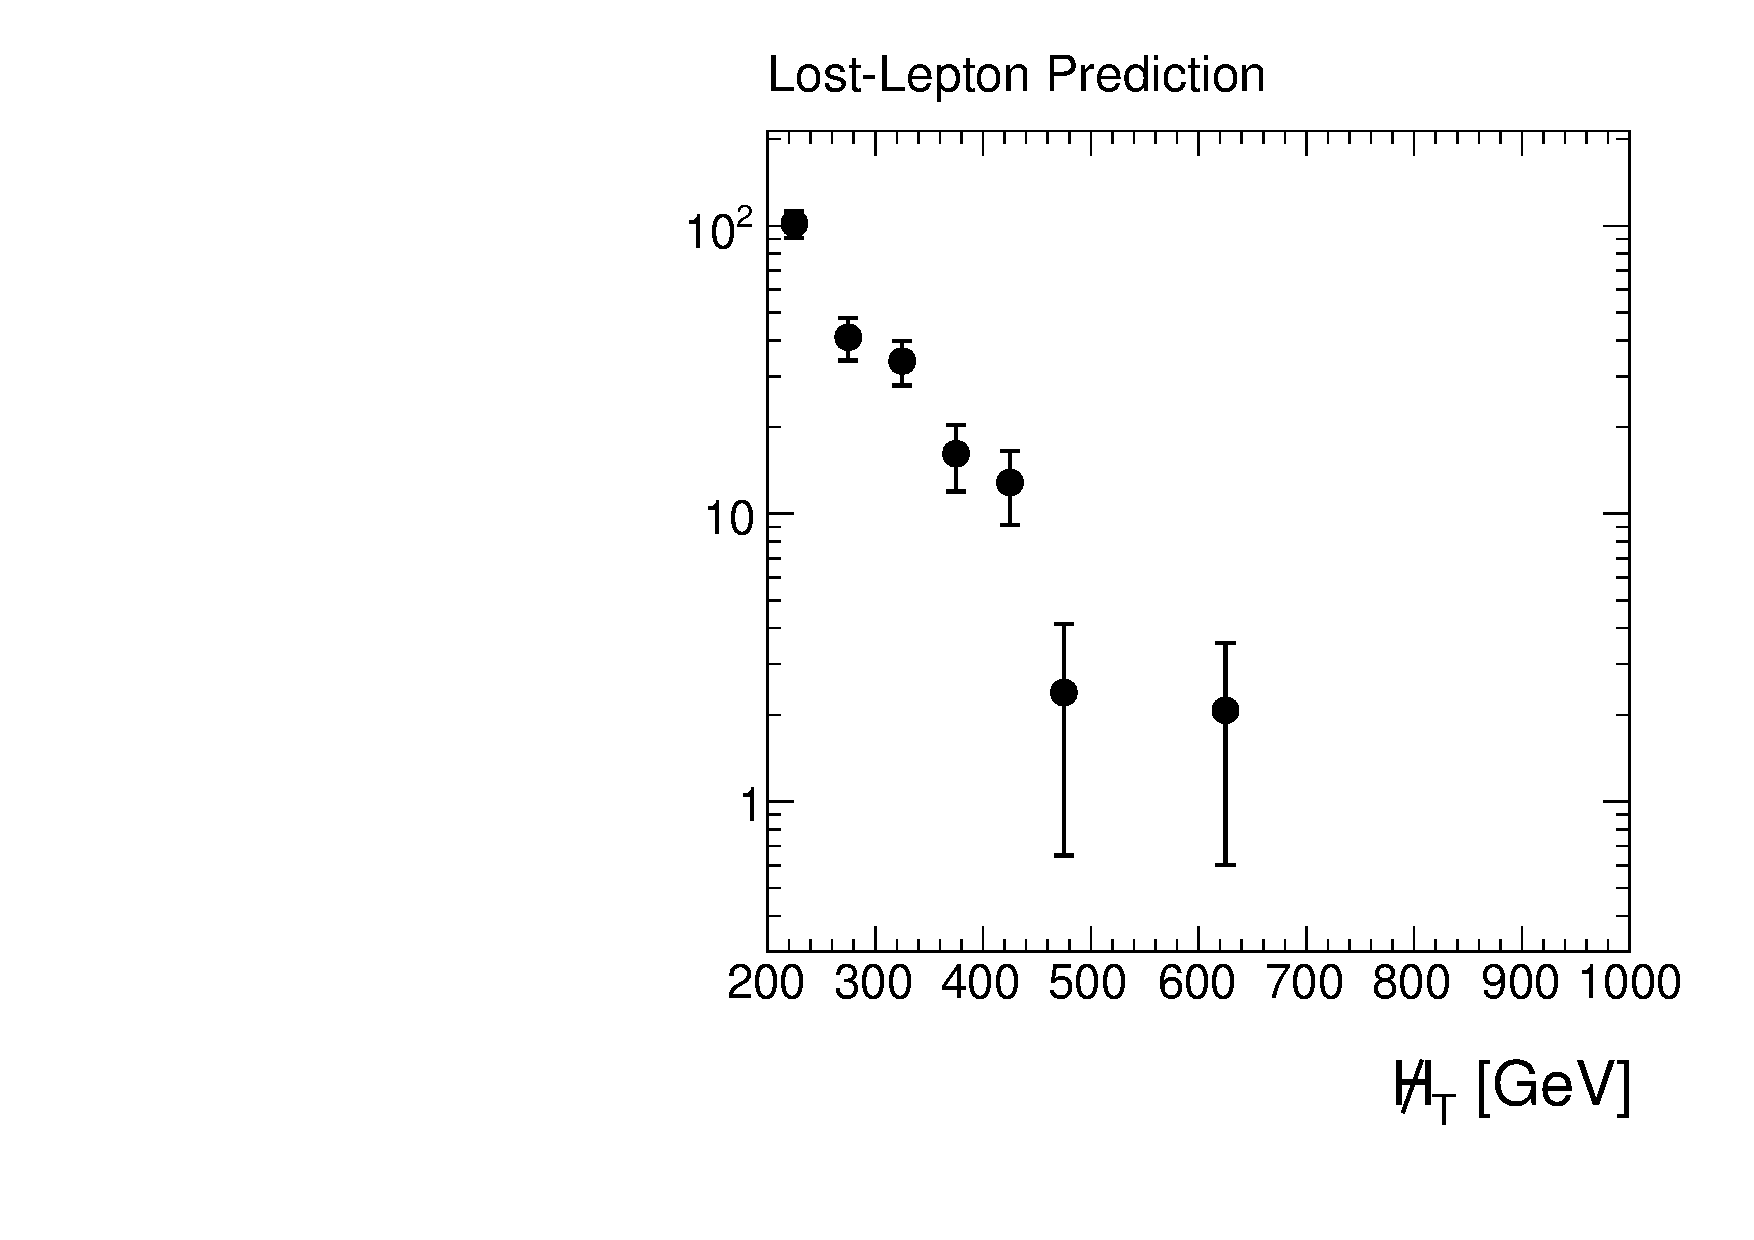
\includegraphics[width = 0.4\textwidth]{plots11/LLPredictionMHT.pdf}
\end{center}

\end{frame}



%- "neues" Ergebnis vs altes (spoiler: Gleich mit homemade gewichten) 
\begin{frame}{Combined Results}

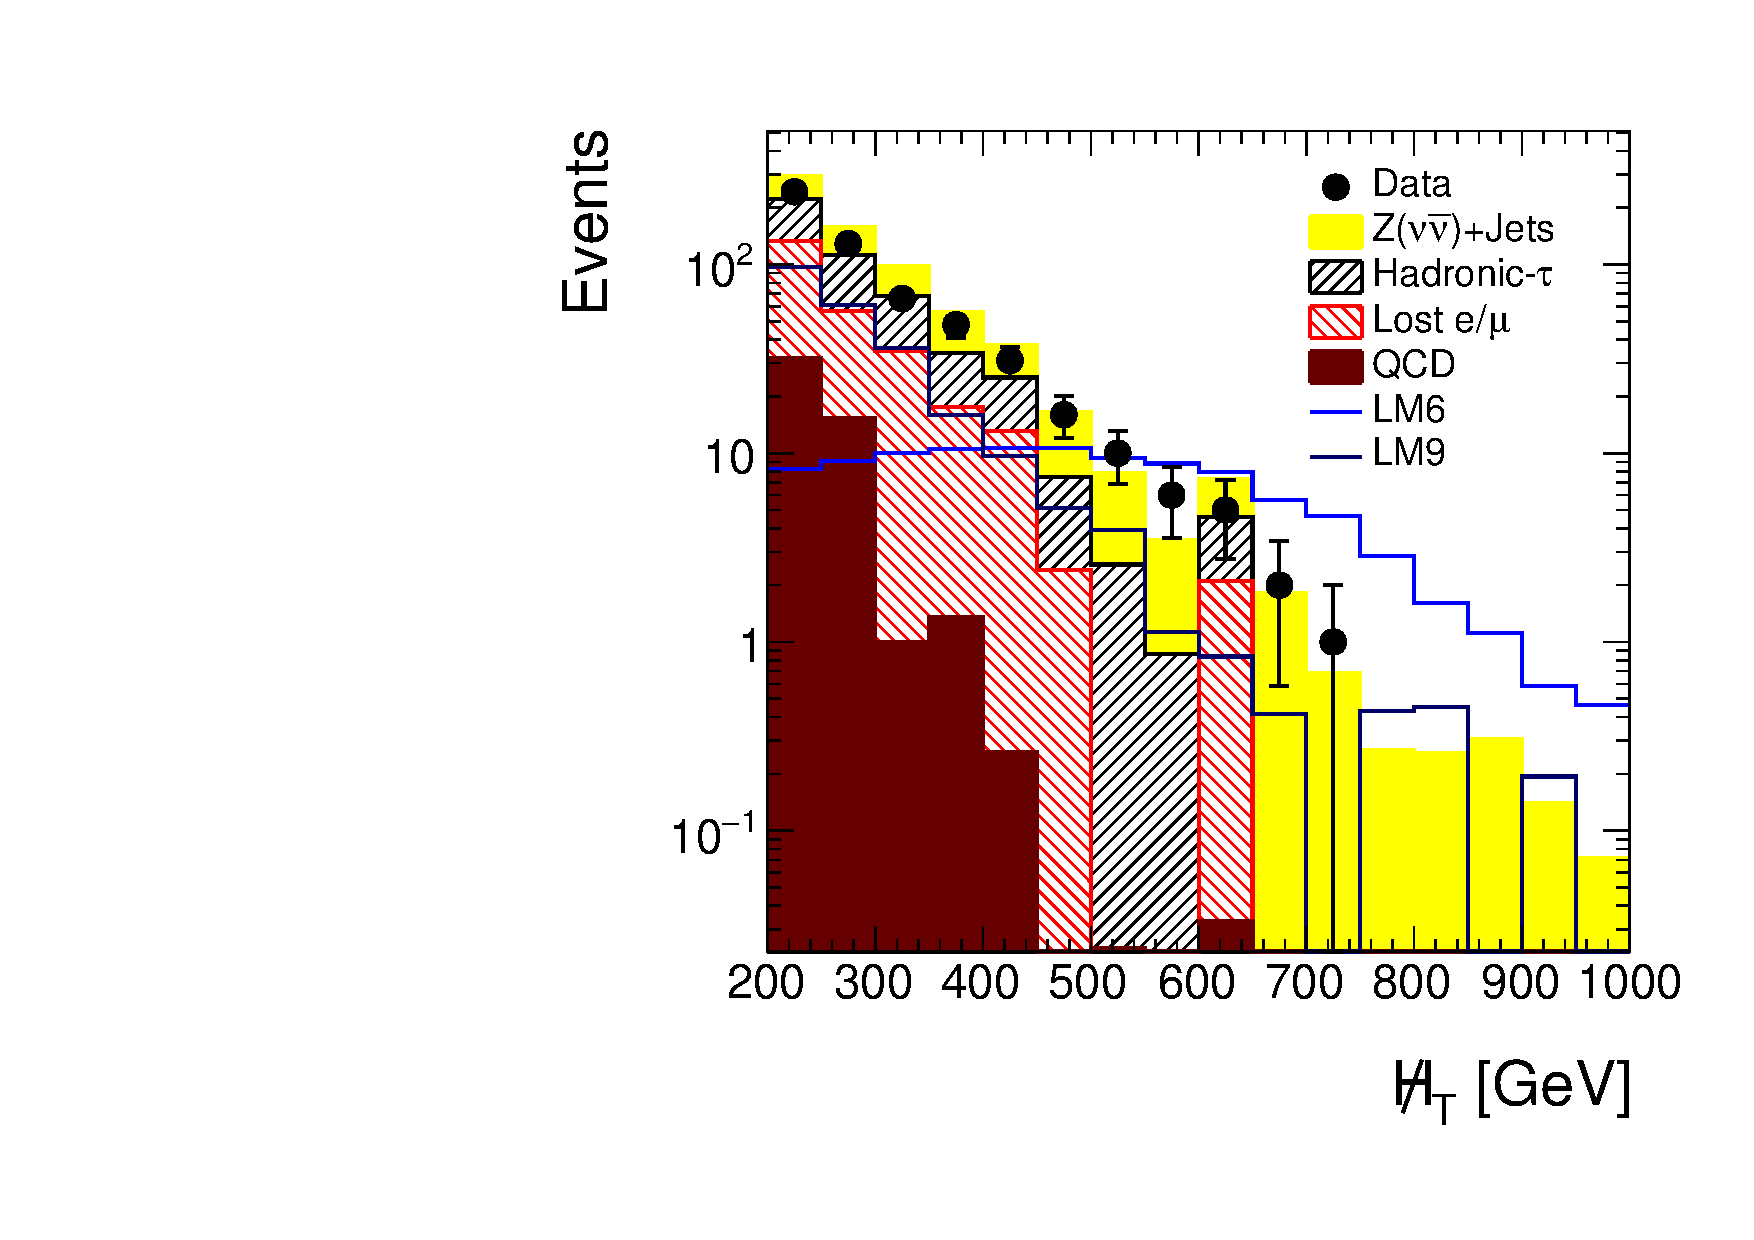
\includegraphics[width = 0.45\textwidth]{plots11/hDataVsBkg_Mht.pdf}
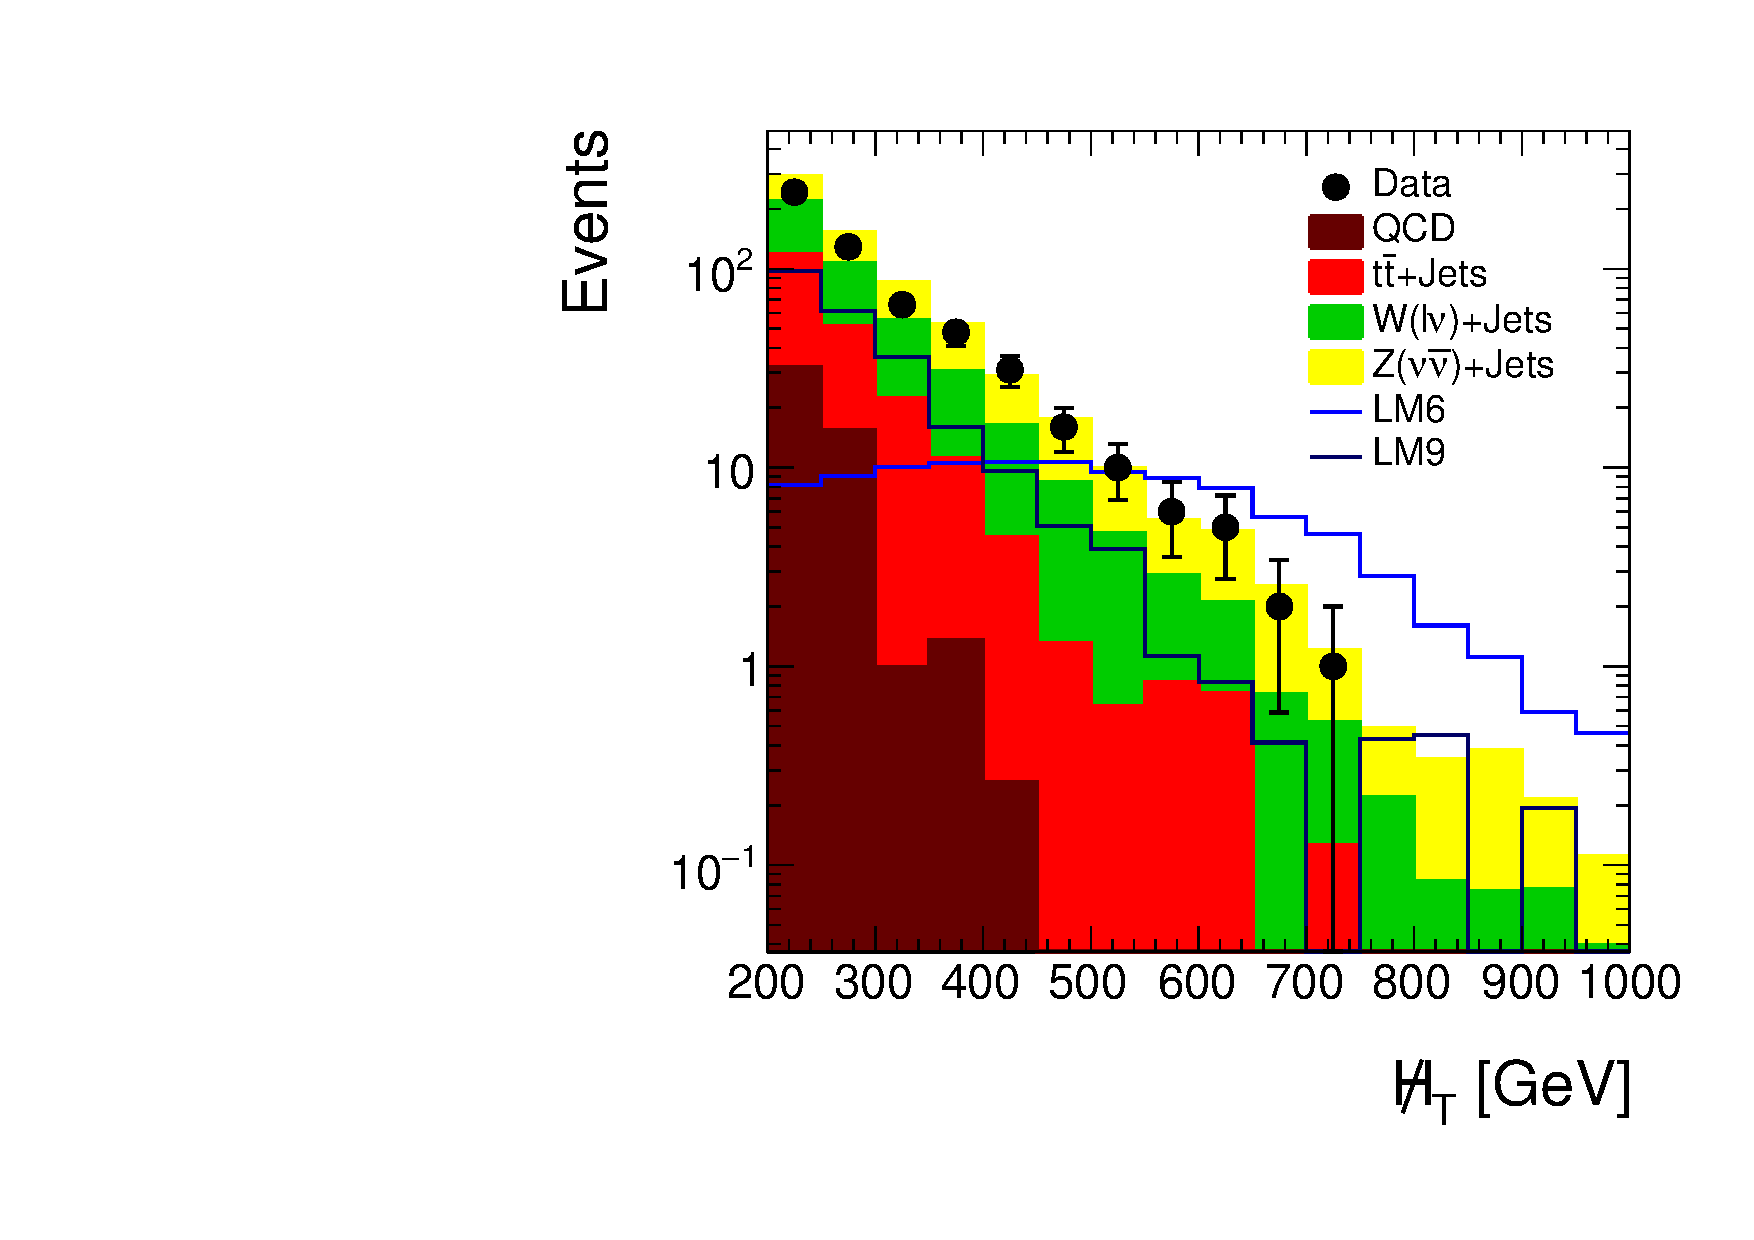
\includegraphics[width = 0.45\textwidth]{plots11/hDataVsMC_Mht.pdf}\\
$\Rightarrow$ still no SUSY found :(
\end{frame} 
